%\documentclass{article} %[twocolumn] 
%\documentclass[Crown, times, sagev]{sagej}
%\documentclass[MCfour, sagev]{sagej}
\documentclass[sagev]{sagej} 

\usepackage{booktabs}
\usepackage{array}
\usepackage{graphicx}
\usepackage{amsmath}
\usepackage{amsfonts}
\usepackage{amssymb}
\usepackage{multirow}
\usepackage{url}
\usepackage{tabularx} 

\setcounter{secnumdepth}{3} %Gives section numbers for cross referencing

% For submissing to Clinical trials: maximum 4,000 words excepting abstract, references, tables and figures; maximum 6 tables or figures.

% Current word count (approx): 4246

\begin{document}

\runninghead{Wilson et al.}

\title{Three-outcome designs for pilot trials with progression criteria}

\author{Duncan T. Wilson\affilnum{1}}%,
%Rebecca E. A. Walwyn\affilnum{1}, 
%Julia Brown\affilnum{1} and 
%Amanda J. Farrin\affilnum{1}}

\affiliation{\affilnum{1}Leeds Institute of Clinical Trials Research, University of Leeds, Leeds, UK} %\\
%\affilnum{2}Centre for Primary Care \& Public Health, Queen Mary University of London, London, UK}

\corrauth{Duncan T. Wilson, Clinical Trials Research Unit, Leeds Institute of Clinical Trials Research, University of Leeds, Leeds, LS2 9JT, UK}
\email{d.t.wilson@leeds.ac.uk}

\begin{abstract}
% 425 words or fewer for Clinical Trials
The decision of if and how to progress to a definitive trial following a pilot study is often guided by progression criteria with three possible outcomes, but there is little methodological work examining how they, or the pilot sample size, should be determined. We review three-outcome designs originally proposed for phase II trials and consider if they can provide a formal statistical framework for pilot trials. We conclude that, from a statistical perspective, there are limited benefits from using three-outcome progression criteria in pilot trials.
\end{abstract}

\keywords{Clinical trial, pilot trial, progression criteria, sample size}

\maketitle

\section{Introduction}\label{sec:introduction}

When there is some uncertainty about the feasibility of a planned randomised clinical trial (RCT), a pilot trial can be conducted in advance. Pilots take the form of a smaller version of the main trial \cite{Eldridge2016}, and can be used to estimate various parameters of interest when deciding if (and how) to progress to the main study. Investing in a pilot trial can identify potential issues at an early stage, making a successful main trial more likely and reducing overall research waste \cite{Morgan2018}.

Progression decisions can be guided by so-called \emph{progression criteria} \cite{Eldridge2016a}. A single two-outcome progression criterion specifies a decision rule which maps the pilot data to a \emph{stop} or \emph{go} outcome. Specifically, the pilot data are used to calculate a statistic, typically an estimate of a parameter of interest, and this statistic is compared against a threshold value. If the statistic exceeds the threshold, the suggested decision is to \emph{go} forward to the main trial; otherwise, to \emph{stop} on the grounds of infeasibility. When progression criteria are specified for several parameters, these can be combined by proceeding to the main trial only if all of the estimates exceed their respective thresholds. It has been recommended that, in addition to being reported in the pilot study manuscript, progression criteria are pre-specified at the protocol stage in agreement with the study funder \cite{NIHR2017, Mbuagbaw2019}.

It has become common for progression criteria to be based on a three-outcome `traffic light' system \cite{Avery2017}. These criteria stipulate two threshold values for a given parameter of interest. If the estimate falls below the lower of these, the decision is to stop (red); if the estimate falls above the higher threshold, the decision is to proceed immediately to the main trial (green); and if the estimate falls between the two thresholds, an intermediate decision is reached (amber). The specific purpose and interpretation of this intermediate can vary, and will depend on the motivation for using the three-outcome system. Three distinct motivations can be found in the methodological literature. Firstly, it has been argued that making strict stop/go decisions based on a single threshold  may lead to an unacceptably high chance of making the wrong decision as a result of sampling variability \footnote{``\emph{\ldots estimates of rates in pilot trials may be subject to considerable uncertainty, so that it is best to be cautious about setting definitive thresholds that could be missed simply due to chance variation. In fact it is becoming increasingly common for investigators to use a traffic light system for criteria used to judge feasibility\ldots}''} \cite{Eldridge2016a}. By allowing for an intermediate result in between \emph{stop} and \emph{go}, the probability of landing in these critical areas, and therefore of making incorrect decisions, will be reduced.

%This argument is paralled in the three outcome literaure, which argue that the designs can improve efficiency and either increase power, or reduce the required sample size.

A second motivation stems from the fact that many aspects (quantitative and qualitative) being studied in a pilot trial are potentially relevant to the progression decision. A three-outcome system will allow immediate \emph{stop} or \emph{go} decisions to be made if the evidence is sufficiently strong with respect to a handful of key parameters, whilst allowing, in the event of a borderline result, the decision to be informed by other data. It has been argued that this system better represents what happens in practice when a two-outcome process is nominally being followed. In that case, although a borderline result will technically dictate a firm \emph{stop/go} decision, this may be overridden in light of other information \cite{Sargent2001}.

A final reason for an intermediate outcome is to provide the flexibility needed to make some adjustment to the intervention or trial design in an attempt to improve the parameter in question and ensure the feasibility of the main trial\footnote{``\emph{In amber situations, there may be remediable issues that would otherwise prevent progression to the main trial but that, if identified early enough, can be addressed to the satisfaction of those reviewing progress in order for the trial to continue to a main trial.}''} \cite{Avery2017}. For example, after observing a mediocre follow-up rate in a pilot trial, we might consider moving from a postal follow-up strategy to one based on contacting the participants over the phone. This approach is somewhat in line with guidance on the development and evaluation of complex interventions \cite{Craig2008} which emphasises the iterative nature of the process and the likely need to adjust the original intervention or trial design before conducting the main trial.

Despite the prevalence of three-outcome progression criteria\cite{Herbert2019}, there is little statistical guidance to help researchers decide how they should be specified. The related question of determining the pilot trial sample size is also undeveloped, with work in this area typically focussing on pilot trials where the primary objective is to estimate the primary outcome variance to inform the main trial sample size calculation. These methods are nevertheless used when this is not the main purpose of the pilot, often in the form of simple `rules-of-thumb' \cite{Browne1995, Teare2014, Whitehead2015}. Three-outcome designs have, however, been proposed for phase II trials of cancer treatments \cite{Kirby2016}. Some of these designs were motivated by the same factors given above, and so may provide a useful framework for the design and analysis of pilot trials with three-outcome progression criteria.

In this paper we consider if, and how, three-outcome phase II designs can be used to determine optimal progression criteria and sample size in pilot trials. We begin by introducing a simple example in Section \ref{sec:example}. In Section \ref{sec:tests} we argue that progression criteria are mathematically equivalent to hypothesis tests, and are best viewed as such. We then review relevant three-outcome phase II trial designs in Section \ref{sec:review}. In Section \ref{sec:methods}, we examine the statistical properties of these designs as applied to pilot trials with progression criteria, and consider whether or not they can help achieve any of the three motivating goals. Finally, we conclude with a discussion in Section \ref{sec:discussion}.

\section{An example}\label{sec:example}

Throughout this article we will refer to a simple example of a pilot trial assessing the probability that a participant in the intervention arm of the main trial will adhere to their prescribed treatment. Specifically, we consider adherence to be measured as a binary outcome, and denote the probability of adherence by $\rho$. Given  $n$ patients in the pilot trial's intervention arm, we then model the number of adherers using a binomial distribution with parameters $\rho, n$. We denote the pilot estimate by $\hat{\rho}$.

We will consider both two- and three-outcome versions of progression criteria. In the two-outcome case, the progression decision is defined by a threshold value $x$, such that
\begin{equation}\label{eqn:two_outcome}
\text{Decision} = 
\begin{cases}
\text{\emph{go}} & \text{ if } \hat{\rho} \geq x \\
\text{\emph{stop}} & \text{ if } \hat{\rho} < x. \\
\end{cases}
\end{equation}

In the three-outcome case, we allow for an additional intermediate result and require two thresholds, $x_0$ and $x_1$:
\begin{equation}\label{eqn:three_outcome}
\text{Decision} = 
\begin{cases}
\text{\emph{go}} & \text{ if } \hat{\rho} \geq x_1 \\
\text{\emph{pause}} & \text{ if } x_0 < \hat{\rho} < x_1 \\
\text{\emph{stop}} & \text{ if } \hat{\rho} < x_0. \\
\end{cases}
\end{equation}
The specific meaning of the intermediate \emph{pause} result will vary depending on the purpose and context of the pilot trial. 

\section{Progression criteria as hypothesis tests}\label{sec:tests}

In order to apply the two-outcome progression criteria of Equation \ref{eqn:two_outcome}, we must choose the sample size $n$ and the threshold $x$. One way to do so is though constructing a hypothesis test as follows. First, we identify a parameter value $\rho_0$ such that if $\rho \leq \rho_0$ we would like to limit the probability of incorrectly making a `go' decision (a type I error) to at most $\alpha^*$. Similarly, we identify $\rho_1$ such that if $\rho \geq \rho_1$ we would like to limit the probability of incorrectly making a `stop' decision (a type II error) to at most $\beta^*$. We then choose values of $n$ and $x$ which minimise $n$ whilst satisfying the type I and II error rate constraints
\begin{align}
\alpha &= \max_{\rho \leq \rho_0} P[ \hat{\rho} > x ~ | ~ \rho] = P[ \hat{\rho} > x ~ | ~ \rho = \rho_0] \leq \alpha^* \\
\beta &= \max_{\rho \geq \rho_1} P[ \hat{\rho} \leq x ~ | ~ \rho] = P[ \hat{\rho} \leq x ~ | ~ \rho = \rho_1] \leq \beta^*,
\end{align}
where we have used the monotonicity of the power function to note that the type I and II error rates will be maximised when $\rho = \rho_0$ and $\rho = \rho_1$ respectively.

Alternatively, we can work backwards and take any given choice for $n$ and $x$ and calculate the resulting error rates for some hypotheses $\rho_0, \rho_1$. In particular, whenever a pilot trial progression criteria is specified in the form of Equation \ref{eqn:two_outcome}, it is mathematically equivalent to a hypothesis test. For example, consider a pilot trial with $n = 15$ participants in the intervention arm and a \emph{stop/go} progression criteria with threshold $x = 10/15$. If we suppose that the null and alternative hypotheses are $\rho_0 = 0.6, \rho_1 = 0.8$ respectively, we see that this design gives type I and II error rates of $\alpha = 0.22$ and $1 - \beta = 0.84$. Alternatively, we can constrain the error rates to, for example, $\alpha^* = 0.05$ and $\beta^* = 0.1$, in which case the smallest possible sample size is $n = 48$ and the corresponding progression threshold is $x = 34/48$. 

The equivalence of two-outcome progression criteria and hypothesis tests suggests the latter can provide a statistical framework for determining the former \cite{Lewis2021a}. This will allow us to express what parameter values would lead to errors of each type, and then subsequently to control the probability of these errors by choosing a sufficient sample size.

\section{Three-outcome phase II trial designs}\label{sec:review}

Just as standard hypothesis testing can be used as a framework for two-outcome progression criteria, three-outcome extensions can be used for the three-outcome progression criteria of Equation \ref{eqn:three_outcome}. We will consider two such extensions, proposed for phase II trials by Sargent \emph{et al.} \cite{Sargent2001} and by Storer \cite{Storer1992}.

The design of Sargent \emph{et al.} defines four operating characteristics relevant to the three-outcome setting. Firstly, a measure akin to the type I error rate $\alpha_a$ is defined as the probability, under the null hypothesis, that the parameter estimate will exceed the upper threshold $x_1$ and thereby lead to a \emph{go} decision. Similarly, a type II error rate $\beta_a$ is given as the probability, under the alternative hypothesis, of the parameter estimate failing below the lower threshold $x_0$ and leading to a \emph{stop} decision. Two further operating characteristics relating to the intermediate outcome are then defined: the probability of obtaining a \emph{pause} decision under then null hypothesis, $\lambda$, and again under the alternative hypothesis, $\gamma$. These operating characteristics are summarised in Table \ref{tab:ocs} and illustrated in Figure \ref{fig:Sarg_ocs}. The authors propose to set constraints on these four operating characteristics and choose $n, x_0, x_1$ to minimise $n$ whilst satisfying these constraints, and they argue that their designs will typically lead to a lower sample size requirement than standard two-outcome alternatives.

\begin{table}
\caption{Operating characteristics for Sargent \emph{et al.} and Storer's three-outcome designs \cite{Sargent2001, Storer1992}.}
\begin{tabularx}{\textwidth}{l l l X}
\toprule
 & Symbol & Equation & Description \\
\midrule
\multirow{9}{*}{\rotatebox[origin=c]{90}{Sargent}} & $\alpha_a$ & $P[ \hat{\rho} > x_1 | \rho = \rho_0]$ & Probability of an immediate \emph{go} decision under the null hypothesis \\
 & $\beta_a$ & $P[ \hat{\rho} \leq x_0 | \rho = \rho_1]$ & Probability of an immediate \emph{stop} decision under the alternative hypothesis \\
 & $\lambda$ & $P[ x_0 < \hat{\rho} \leq x_1 | \rho = \rho_0]$ & Probability of a \emph{pause} decision under the null hypothesis \\
 & $\delta$ & $P[ x_0 < \hat{\rho} \leq x_1 | \rho = \rho_1]$ &  Probability of a \emph{pause} decision under the alternative hypothesis \\
 &&& \\
\multirow{10}{*}{\rotatebox[origin=c]{90}{Storer}} & $\alpha_b$ & $P[ \hat{\rho} > x_0 | \rho = \rho_0]$ & Probability of not obtaining an immediate \emph{stop} decision under the null hypothesis \\
 & $\beta_b$ & $P[ \hat{\rho} \leq x_1 | \rho = \rho_1]$ & Probability of not obtaining an immediate \emph{go} decision under the alternative hypothesis \\
 & $\gamma_L$ & $P[ \hat{\rho} \leq x_0 | \rho = \rho_m]$ & Probability of an immediate \emph{stop} decision when $\rho = \rho_m$ \\
 & $\gamma_U$ & $P[ x_1 < \hat{\rho} | \rho = \rho_m]$ &  Probability of an immediate \emph{go} decision when $\rho = \rho_m$ \\
\bottomrule
\end{tabularx}
\label{tab:ocs}
\end{table}

\begin{figure}
\centering
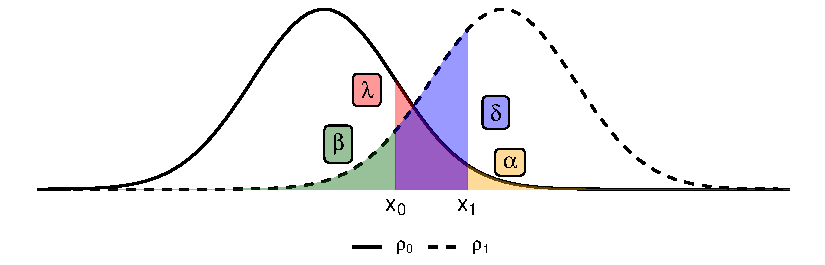
\includegraphics[scale=0.8]{./figures/Sarg_ocs}
\caption{Graphical illustration of the perating characteristics for Sargent \emph{et al.}'s three-outcome design \cite{Sargent2001}. The curves represents the sampling distribution of the estimate under different values of the parameter $\rho$.}
\label{fig:Sarg_ocs}
\end{figure}

An alternative three-outcome design proposed by Storer \cite{Storer1992} takes the same basic approach, but with a different set of four operating characteristics. Here, the type I error rate $\alpha_b$ is taken to be the probability of exceeding the lower threshold, $x_0$, under the null; and similarly the type II error rate $\beta_b$ is now the probability of failing to exceed the upper threshold under the alternative. The remaining two operating characteristics are the probabilities of incorrectly obtaining a \emph{stop} or a \emph{go} decision when the true parameter is at some midpoint $\rho_m \in (\rho_0, \rho_1)$. These operating characteristics, denoted by $\gamma_L$ and $\gamma_U$ respectively, reflects the motivation of the design to \emph{encourage} an intermediate outcome when the true parameter value is between the null and alternative. The operating characteristics are summarised in Table \ref{tab:ocs} and illustrated in Figure \ref{fig:Stor_ocs}, where we follow the author's suggestion to set $\rho_m = (\rho_1 - \rho_0)/2$.

\begin{figure}
\centering
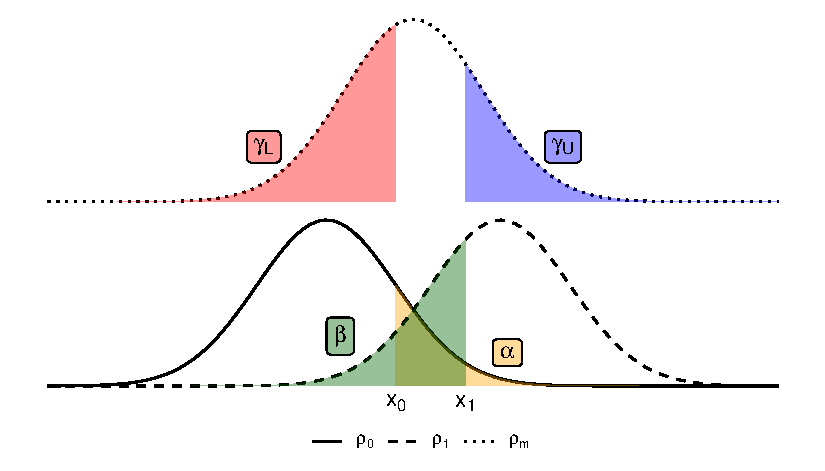
\includegraphics[scale=0.8]{./figures/Stor_ocs}
\caption{Graphical illustration of the operating characteristics for Storer's three-outcome design\cite{Storer1992}. The curves represents the sampling distribution of the estimate under different values of the parameter $\rho$.}
\label{fig:Stor_ocs}
\end{figure}

Considering the proposal of Sargent \emph{et al.}, we note that the measure $\alpha_a$ does not fully capture the probability of making a type I error \footnote{Sargent \emph{et al.}  state that ``We  can interpret $\alpha$ in the usual  manner,  i.e., the  maximum probability of making an erroneous decision by rejecting the null hypothesis when in fact it is true''} since a decision to progress to the main trial can be arrived at in two ways: directly, by obtaining $\hat{\rho} > x_1$; or indirectly, by first obtaining an intermediate result $x_0 < \hat{\rho} < x_1$ and then deciding to proceed. To capture these situations, first define the following:
\begin{align}
\eta_0 &= P[\text{decide to \emph{go}} ~|~ \rho = \rho_0, x_0 < \hat{\rho} \leq x_1] \\
\eta_1 &= P[\text{decide to \emph{stop}} ~|~ \rho = \rho_1, x_0 < \hat{\rho} \leq x_1].
\end{align}
For example, $\eta_0$ is the probability of making a \emph{go} decision following an intermediate result and when the true parameter value is $\rho_0$. The probability of making a \emph{go} decision when $\rho = \rho_0$, then, is not $\alpha_a$ but
$$
\alpha = \alpha_a + \eta_0 \lambda.
$$
Similarly, the type II error rate is
$$
\beta = \beta_a + \eta_1 \delta.
$$
These operating characteristics have been suggested previously in the context of multi-armed screening trials \cite{Sargent2001a, Dehbi2020}. Under this reformulation, an optimal three-outcome design can be found by first estimating the probabilities $\eta_0, \eta_1$, then setting constraints on the reformulated type I and II error rates $\alpha, \beta$, and finally searching for the values of  $n, x_0, x_1$ which minimise $n$ whilst satisfying the constraints. For simplicity we will assume that $\eta_0 = \eta_1 = \eta$; that is, the probability of eventually making the wrong decision following an intermediate result is the same when $\rho = \rho_0$ as when $\rho = \rho_1$. The operating characteristics $\delta$ and $\lambda$ are no longer relevant, because an intermediate result under $\rho_i$ is only an error in as much as it may lead to the wrong decision with probability $\eta$. That is, we do not require a mechanism to keep the probability of this outcome low, as this will be taken care of automatically when constraining $\alpha$ and $\beta$.

A similar argument applies when considering Storer's method, where we can replace the operating characteristics $\alpha_b, \beta_b$ with $\alpha$ and $\beta$. As the operating characteristics $\gamma_L, \gamma_U$ are designed to encourage an intermediate outcome under $\rho_m$, rather than limit it as in the method of Sargent \emph{et al.}, we keep these in our reformulation. Thus, an optimal three-outcome design under the reformulated Storer method can be found by estimating the probabilities $\eta_0, \eta_1$, setting constraints on $\alpha, \beta, \gamma_L$ and $\gamma_U$, and finally searching for the values of  $n, x_0, x_1$ which minimise $n$ whilst satisfying the constraints. 

For simplicity, we will assume that the cost of an incorrect \emph{stop} or \emph{go} decision under $\rho = \rho_m$ are the same, and replace the two error rates $\gamma_U, \gamma_L$ by the single error rate
$$
\gamma = \gamma_L + \gamma_U,
$$
the probability of making an incorrect conclusive decision of either type. Note that the reformulated method of Sargent \emph{et al.} is a special case of this method when we set the trivial constraint $\gamma \leq 1$, and so we have a single unified framework for designing and analysing three-outcome studies.

\section{Three-outcome designs for progression criteria}\label{sec:methods}

As noted in Section \ref{sec:introduction}, adding a third outcome to pilot trial progression criteria has been motivated on grounds of i) statistical efficiency; ii) the need to incorporate other information into progression decisions; and iii) the ability to make modifications to the intervention or the trial design before commencing the main trial. In this section we discuss if the three-outcome design framework described in Section \ref{sec:review} can be used to address these goals.

\subsection{Statistical efficiency}\label{sec:efficiency}

Sargent \emph{et al.} show that three-outcome designs based on the operating characteristics given in Table \ref{tab:ocs} will have a lower sample size than an optimal two-outcome design, providing $\lambda$ and/or $\delta$ are allowed to be greater than 0. For example, take $\rho_0 = 0.5$ and $\rho_1 = 0.7$. A two-outcome design will require $n = 53$ to ensure $\alpha \leq 0.05$ and $\beta \leq 0.1$. In contrast, by allowing $\lambda \leq 0.1$ and $\delta \leq 0.1$ in a three-outcome design, we can obtain $\alpha_a \leq 0.05$ and $\beta_a \leq 0.1$ with only $n = 42$, suggesting three-outcome designs are indeed more efficient \cite{Sargent2001, Hong2007}. However, this apparent advantage breaks down when using the reformulation given in Section \ref{sec:review}. Using that method, we found optimal sample sizes for this example problem over the range $0 \leq \eta \leq 0.5$ and using the constraints $\alpha \leq 0.05, \beta \leq 0.1, \gamma \geq 0$. These are plotted in Figure \ref{fig:eta_ns}.

\begin{figure}
\centering
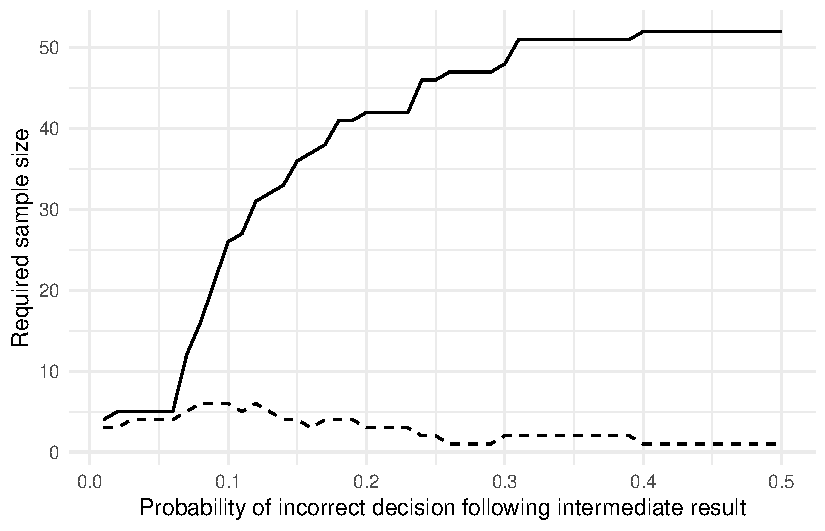
\includegraphics[scale=0.8]{./figures/eta_ns}
\caption{Minimum required sample size for a three-outcome design as a function of $\eta$ (solid line), along with the corresponding size of the intermediate zone $x_1 - x_0$ (dashed line).}
\label{fig:eta_ns}
\end{figure}

When $\eta = 0.5$, in which case we can only guess at the correct decision following an intermediate result, the optimal sample size is $n = 52$. \footnote{We might have expected the three- and two-outcome designs to coincide at this point, and indeed this is the case if we employ a normal approximation for $\hat{\rho}$. When using exact binomial probabilities, as we have done here, the optimal three-outcome design has $x_0 = 31, x_1 = 32$, in comparison to the $x = 32$ of the two-outcome design. This suggests the true optimal $x$ for a two-outcome design lies in the interval $(31, 32)$} We have not considered $\eta > 0.5$ as this represents a decision making ability worse than random, in which case the optimal design remains the usual two-outcome design.

Figure \ref{fig:eta_all} shows that in order to achieve a meaningful reduction in sample size, a low value of $\eta$ is required. For example, for a 20\% reduction from the $n = 53$ two-sample design down to $n = 42$, we would require $\eta = 0.2$. That is, we must be confident that following an intermediate result, but with a true $\rho = \rho_i (i = 0,1)$, we will make the correct progression decision with a probability of 0.8. In the context of our simple one-parameter example, the estimate $\hat{\rho}$ is a sufficient statistic for $\rho$ and so we cannot hope to obtain any other information relevant to this particular judgement. This would lead to $\eta = 0.5$, in which case the optimal three-outcome design will reduce to a two-outcome design.

We may expect $\eta < 0.5$ if another outcome in the trial, correlated with the outcome being assessed with the progression criteria, is going to be used when making decisions following an intermediate result. The extent of this will depend, however, on the strength of the correlation, and so may be hard to judge at the design stage. To explore the implications of incorrectly assuming $\eta < 0.5$, we took each of the optimal designs found over the range $0 \leq \eta \leq 0.5$ and calculated their type I and II error rates when $\eta = 0.5$. These error rates are plotted in Figure \ref{fig:eta_true_ocs}. We find that error rates will be substantially inflated whenever the assumed $\eta$ was sufficiently small as to lead to a meaningful reduction in sample size. For example, if we incorrectly assume $\eta = 0.2$ when in fact $\eta = 0.5$, the `optimal' design will lead to actual type I and II error rates of 0.081 and 0.155, rather than the nominal 0.05 and 0.1.

\begin{figure}
\centering
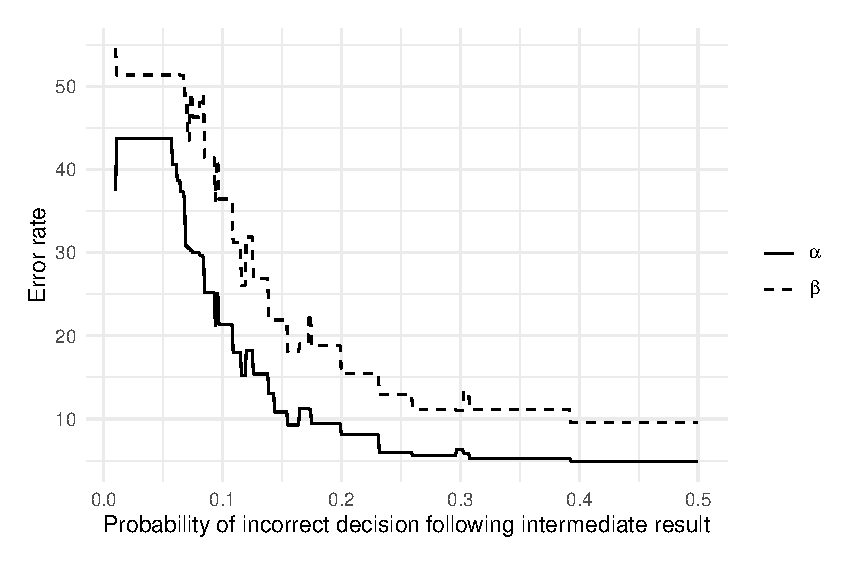
\includegraphics[scale=0.8]{./figures/eta_true_ocs}
\caption{Type I (solid line) and II (dashed line) error rates of optimal three-outcome designs for a range of assumed $\eta$, when in fact $\eta = 0.5$.}
\label{fig:eta_true_ocs}
\end{figure}

% 0.20 42 24 27 0.04541903 0.09349647   3 0.08087869 0.1548251

Given the challenges of estimating $\eta$ and the implications of doing it badly, we follow previous suggestions \cite{Sargent2001a, Dehbi2020} that a default assumption of $\eta = 0.5$ is appropriate and, therefore, three-outcome progression criteria are not suitable for improving statistical efficiency in pilot trials.

% NOTE - we might imagine that in practice, making a decision after an amber result will just mean using another threshold in the amber region, thus reducing everything down to a two-outcome test.

\subsection{Incorporating other information}\label{sec:information}

We have argued that, without strong assumptions, using other sources of information to make progression decisions via an intermediate result will not improve statistical efficiency. We may, nevertheless, want to use such a procedure to allow this other information to inform the progression decision, rather then being ignored completely. In this case we can encourage the design to have an appropriate intermediate zone through constraints on the operating characteristics $\gamma_L, \gamma_U$ defined in Table \ref{tab:ocs}, limiting the chance of making a conclusive \emph{stop} or \emph{go} decision when $\rho = \rho_m$. With $\rho_0 = 0.5, \rho_1 = 0.7, \alpha \leq 0.05$ and $\beta \leq 0.1$ as before, we set $\rho_m = (\rho_1 - \rho_0)/2 = 0.6$ and found optimal designs for a range of $\gamma^*$, where $\gamma_L, \gamma_U \leq \gamma^*$. The sample size of these designs are plotted in Figure \ref{fig:gamma_ns}.

\begin{figure}
\centering
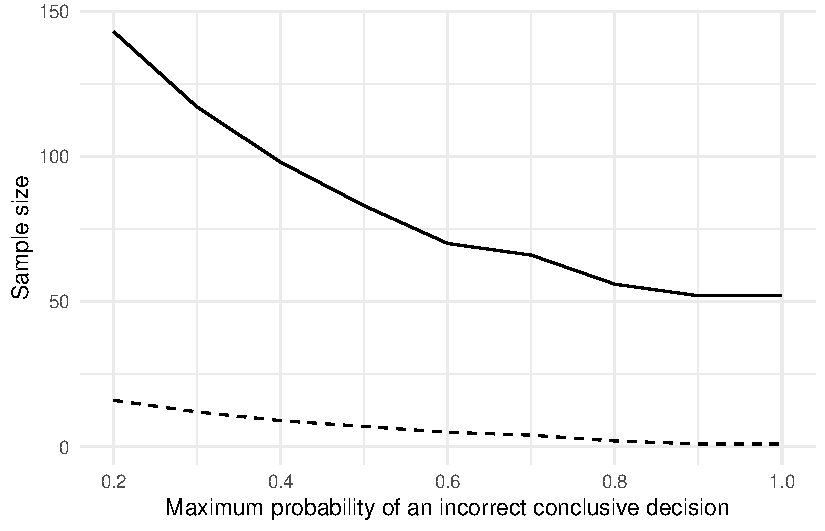
\includegraphics[scale=0.8]{./figures/gamma_ns}
\caption{Minimum required sample size for a three-outcome design as a function of $\gamma$ (solid line), along with the corresponding size of the intermediate zone $x_1 - x_0$ (dashed line).}
\label{fig:gamma_ns}
\end{figure}

When we set $\gamma^* = 1$, no intermediate zone is required and so the optimal design is the usual two-outcome design. As we decrease the nominal level on this constraint, we permit a smaller probability of obtaining an conclusive result when $\rho = \rho_m$. This leads to an increasing width of the intermediate zone, alongside an increasing sample size. The required increase in sample size beyond the two-outcome design can be substantial. For example, to ensure a maximum 40\% chance of obtaining a conclusive result when $\rho = \rho_m$, we must increase the sample size from $n = 53$ to $n = 98$. 

Providing the associated increase in sample size is considered worthwhile, we conclude that three-outcome designs could be used in pilot trials to ensure other information can be considered in the event of a `borderline' value in the parameter of interest, with some desired probability.

\subsection{Allowing for adjustments}

A final rationale for an intermediate outcome in pilot trials is to enable some modifications to be made prior to commencing the main trial. These could be adjustments to the trial design (e.g. to improve recruitment) or to the intervention itself (e.g. to improve adherence). In this case, the intermediate \emph{pause} decision represents making these modifications and then proceeding to the main trial. We will distinguish between cases where the nature and effect of this adjustment is known at the design stage, and when it is not.

\subsubsection{Known adjustment effect}

Denote the effect of the anticipated adjustment by $\tau$, and assume this is fixed and known \emph{a priori}. Thus, if the true unadjusted adherence rate is $\rho$ and an intermediate outcome $x_0 < \hat{\rho} \leq x_1$ is observed, the adjusted adherence rate in the main trial will be $\rho + \tau$. To define operating characteristics in this context, we need to clarify the meaning of type I and II errors. We propose that a type I error occurs whenever we conduct the main trial with an adherence rate less than $\rho_0$, regardless of whether or not an adjustment has been made. Similarly, we propose that  type II error occurs when we do not conduct the main trial despite the (possibly adjusted) adherence rate being greater than $\rho_1$. We formally define these type I and II error rates by
\begin{equation}\label{eqn:adj_ocs}
\begin{aligned}
\alpha &= \max ~ (Pr[ \hat{\rho} > x_1 ~|~ \rho = \rho_0 ], Pr[ x_0 \leq \hat{\rho} \leq x_1 ~|~ \rho = \rho_0 - \tau]) \\
\beta &=\max ~ (Pr[ \hat{\rho} \leq x_0 ~|~ \rho = \rho_1 - \tau ], Pr[ \hat{\rho} > x_1 ~|~ \rho = \rho_0, \tau > \rho_1 - \rho_0]).
\end{aligned}
\end{equation}
The type I error rate is the largest of the probability of obtaining a \emph{go} decision when $\rho = \rho_0$ and the probability of obtaining an \emph{adjust} decision when $\rho + \tau = \rho_0$. The type II error rate is the largest of the probability of obtaining a \emph{stop} decision when $\rho = \rho_1 - \tau$ and the probability of obtaining a \emph{go} decision when $\rho = \rho_0$, but the effect of the adjustment is sufficient such that $\rho + \tau > \rho_1$. 

Considering the same problem as before ($\rho_0 = 0.5, \rho_1 = 0.7, \alpha^* = 0.05, \beta^* = 0.1$) we found optimal designs for a range of known adjustment effects spanning $\tau \in [0, 0.5]$. The required sample size of these designs is illustrated in Figure \ref{fig:tau_ns}. When adjustments have no effect ($\tau = 0$), the optimal three-outcome design reduces to the usual \emph{stop/go} two-outcome design, with $n = 53$ and $x_0 = x_1 = 32$. As $\tau$ increases, the required sample size initially increases with it before decreasing again. At the extreme of $\tau = 0.5$, in which case adjustment will lead to an empty set for the null hypothesis (since $\rho + \tau > \rho_0 = 0.5$), the optimal three-outcome design is to always arrive at an intermediate result and make the adjustment.

\begin{figure}
\centering
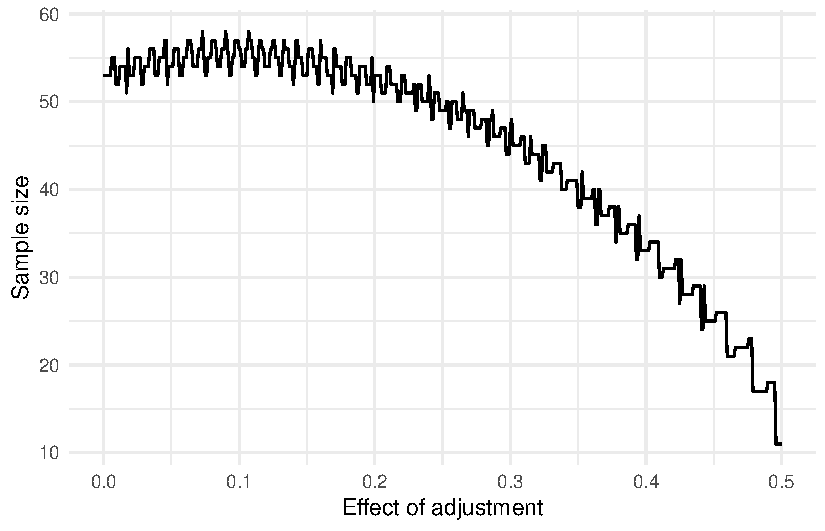
\includegraphics[scale=0.8]{./figures/tau_ns}
\caption{Minimum required sample size for a three-outcome design as a function of the known adjustment effect $\tau$.}
\label{fig:tau_ns}
\end{figure}

\subsubsection{Unknown adjustment effect}

Assuming the adjustment effect $\tau$ is known \emph{a priori} will not always be tenable. On the contrary, a primary goal of many pilot trials is to identify \emph{unforeseen} problems, and solutions to these. In this context, pre-specifying an upper threshold $x_1$ may make sense as this can help identify cases which are feasible enough, without modification, to proceed to the main trial. In contrast, the lower threshold $x_0$ appears arbitrary and may force inappropriate decisions. For example, if $x_0$ is set too high, we may be led to a \emph{stop} decision (i.e. $\hat{\rho} \leq x_0$) but believe, based on what was seen in the pilot, that a certain modification would lead to an adjusted rate greater than $\rho_1$. 

To explore this further we evaluated the actual type I and II error rates for a range of adjustment effects $\tau$ when the optimal three-outcome design based on an assumed $\tau = 0.1$ is used. These error rates are illustrated in Figure \ref{fig:tau_ocs}. We find that when $\tau < 0.1$, in which case our initial estimate of the effect of adjustment was too optimistic, the type I error rate of the trial rapidly increases. This increase is offset, to some extent, by a reduction in the type II error rate. Conversely, for $\tau > 0.1$, we find a rapid increase in the type II error rate. In this case, however, the type I error rate does not decrease substantially. 

\begin{figure}
\centering
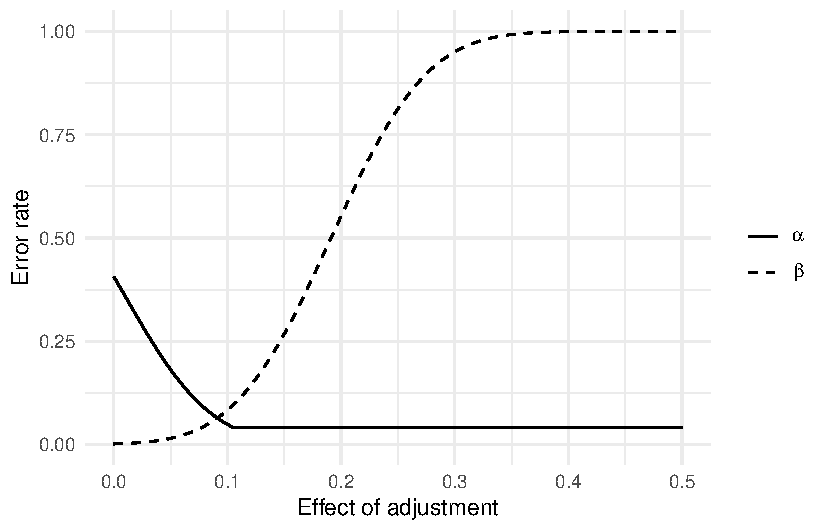
\includegraphics[scale=0.8]{./figures/tau_ocs}
\caption{Type I (solid line) and II (dashed line) error rates for a range of true adjustment effects $\tau$, when designed assuming $\tau = 0.1$.}
\label{fig:tau_ocs}
\end{figure}

We conclude that for three-outcome progression criteria to be useful in this context, the effect of the anticipated adjustment must be known (or at least estimated with little error) at the design stage. Given the difficulties in making such predictions, and the implications of being mistaken, we do not recommend three-outcome progression criteria as a way to facilitate making adjustments to the intervention or trial design following the pilot trial.

\section{Discussion}\label{sec:discussion}

We have shown how the three-outcome progression criteria commonly used in pilot trials can be viewed as three-outcome hypothesis tests, and described how related clinical trial designs from the phase II setting can be used (with some reformulation) to optimise these criteria and the pilot sample size. This allowed for a formal comparison to be made between three- and two-outcome designs for pilot trials, the results of which led us to conclude that three-outcome designs offer limited benefits. In particular, we have shown that three-outcome designs do not improve efficiency, and can help us decide on adjustments to the intervention or main trial design if the effect of these adjustments are known in advance. Although three-outcome designs were found to allow other sources of information to feed into progression decisions, this came at a substantial cost in terms of the pilot trial sample size.

As an alternative means to improve efficiency in pilot trials, adaptive designs incorporating one or more interim analysis may be useful. These would allow the pilot trial to finish early if interim data gave a sufficiently strong indication of feasibility (or lack thereof). The terminal progression criteria in such an adaptive design could be made three-outcome to allow other information to be incorporated at that stage, and indeed this aligns with Sargent et al.'s \cite{Sargent2001} proposal which included both one and two stage versions of their design. 

To determine if and how the intervention or trial design should be adjusted before the main trial, one could consider a multi-arm pilot trial where each arm implements a different proposed adjustment. This would then inform which adjustment, if any, should be implemented for the main trial. A multi-arm trial will require a larger sample size than a standard two-arm pilot, but this may be mitigated against somewhat by incorporating interim analyses in a Multi-Arm Multi-Stage (MAMS) design. Alternatively, a factorial pilot trial could be used to identify the optimal selection of adjustments to take forward. These solutions would help address the problem of not knowing the effect of some proposed adjustments, but would still require their nature to be known in advance. When a new adjustment is proposed following the pilot trial, undertaking a second pilot to establish that it works as expected may be the best course of action. A similar strategy has been suggested in the context of phase II drug trials \cite{Brown2012}.

An alternative approach to meeting these objectives is to design and analyse the pilot trial under a Bayesian framework\cite{Hampson2017, Wilson2021}. This could improve efficiency by allowing external information or expert knowledge to be incorporated, and would enable a flexible approach to analysis that does not require adherence to pre-specified decision rules. Willan and Thabane \cite{Willan2020} do not consider the question of optimising pilot sample size, but show through an example how a Bayesain analysis of pilot data can help quantify uncertainty around feasibility parameters and use their posterior distributions to design the main trial. 

One conclusion of this work is that standard two-outcome hypothesis tests should be used to determine progression criteria and the pilot trial sample size. The standard approach to this requires a null and alternative hypothesis to be specified, alongside constraints on type I and II error rates which refelct the consequences of these errors. An alternative approach is to instead determine the parameter value at which we would be indifferent between making \emph{stop} and \emph{go} and set the progression criteria threshold to that same value, leading to a test with 50\% power at that point. The sample size can then be chosen to give a desired probability of progression at some other point in the parameter space such as the point null hypothesis \cite{Willan1994}. It seems plausible that this is how progression criteria are currently determined in practice.

Although our findings will apply equally to internal and external pilot trials, the error rates of the final analysis of an internal pilot may be affected by a formal interim analysis of a correlated endpoint such as adherence. Finally, we expect our conclusions to carry over from the univariate setting considered here to the more general multivariate setting, where several progression criteria are applied simultaneously, although it has been shown that such multivariate tests may be counter-intuitively inefficient \cite{Wilson2021a}.

\begin{acks}
Acknowledgements.
\end{acks}

\begin{dci}
The Authors declare that there is no conflict of interest.
\end{dci}

\begin{funding}
This work was supported by the Medical Research Council [grant number MR/N015444/1].
\end{funding}

\bibliographystyle{SageV}
\bibliography{C:/Users/meddwilb/Documents/Literature/Databases/DTWrefs}


\end{document}

MDG:

1) Pilot PCs - example of adherence, from two to three outcomes (example PCs and decision rules)
2) Rationale for three-outcome PCs (efficiency, other info, adjustments)
2) Two-outcome PCs as hypothesis tests. Figure of sampling distribution.
3) Three-outcome phase II designs. Sargent and Storer OCs, motivations, and implications. Figures of sampling distributions.
4) Re-formulation of three-outcome designs. Equations showing new alpha.
5) Efficiency - needs high prob of correct decision making. Figure.
6) Other information - needs an inflated sample size. Figure.
7) Making adjustments - needs effect of adjustment to be known. Figure.
8) Discussion - PCs as tests; Alternative frameworks (precision, Bayesian); Adaptive designs (help efficiency whilst allowing other info, no help for adjustments); Multivariate PCs. 





